\leadchapter{
Decovart abstract!
}
\chapter[DeCovarT: a holistic Bayesian network][DeCovarT: a holistic Bayesian network]{Article 4: DECOVART, a robust deconvolution algorithm exploiting transcriptomic networks}
\label{chap:decovart-algo}

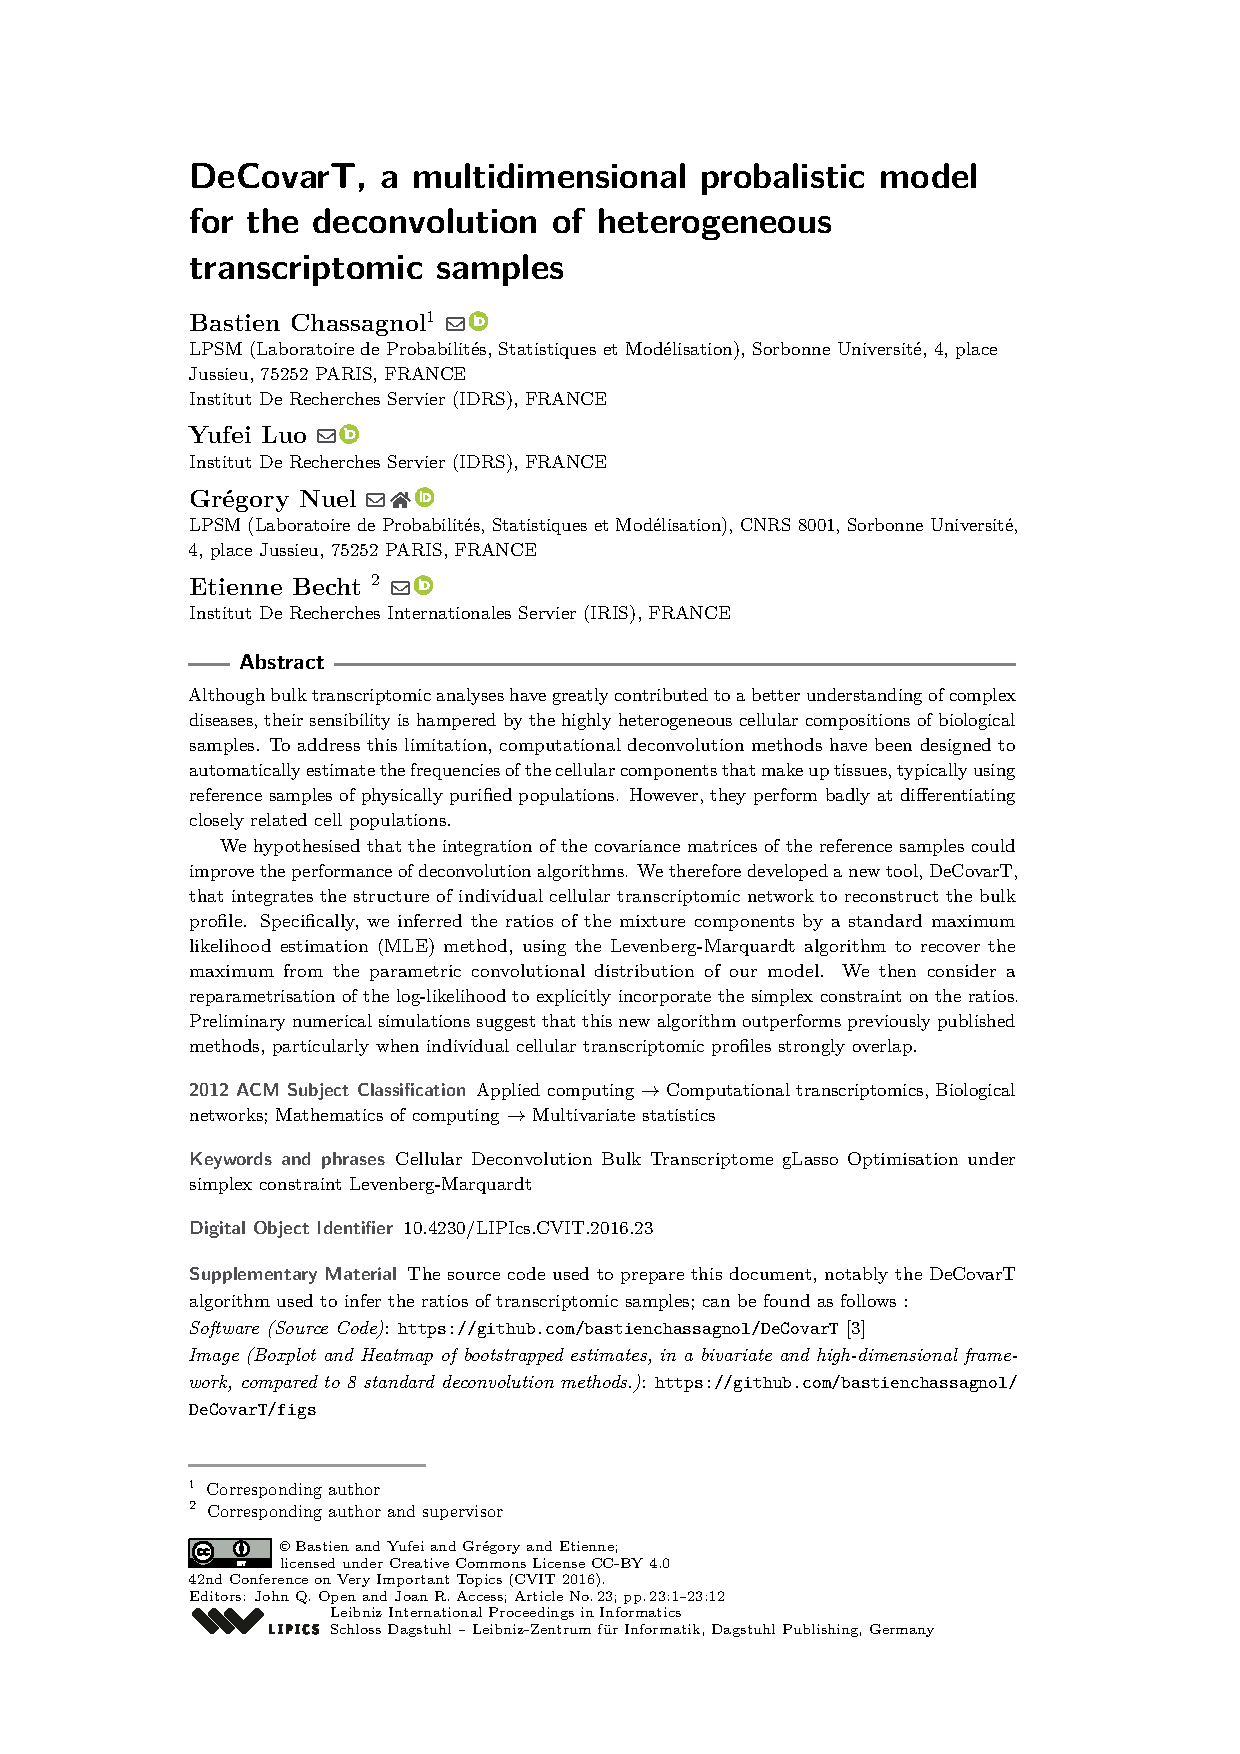
\includepdf[nup=1x1, pages={1-8}]{DeCovart_WABI.pdf}

\section[Deconvolution perspectives][Deconvolution perspectives]{Opinion expert: is the development of scRNA-Seq techniques the death knell for further development of cellular deconvolution methods?}
\label{sec:perspective-deconvolution}

The short answer is no, particularly for applications involving the reconstruction of cellular composition in a temporal and spatial context using \acrfull{st} methods. As discussed in subsection \Cref{subsec:single-cell-spatial-transcript}, there are currently no \acrshort{st} implementations achieving the sequencing of tissue samples at the single cell resolution level, let alone matching the depth and coverage of \acrshort{scrna} methods. 

Indeed, \emph{mismatch}, namely the discrepancy between the cell types detected in single-cell RNA sequencing and the ones spotted in spatial transcriptomics, is . Broadly, mismatch can result from errors in the pre-sequencing steps and in the post-sequencing analysis. Pre-sequencing mismatch can stem from \textit{sampling bias} of the tissue section (lower depth with spatial barcoding or lower coverage or access to intertwined tissue structures with HPRI) or from an artificial stimuli perturbing the cellular expression profile (stress response, or less likely, alteration of cell phenotype due to the disruption of \textit{in situ} spatial dynamics resulting from tissue dissociation). Indeed, it was previously found in 106 that some cell types were highly sensitive to disassociation and do not survive the \acrshort{scrna} workflow, while still present in spatial data. Regarding post sequencing mismatch, it may result from a wrong calibration of the number of population subtypes identified from the clustering of scRNA-Seq datasets.


\emph{Mapping} (see \Cref{subsec:sc-and-st} for details) and \emph{deconvolution} algorithms are key computational tools in alleviating this mismatch issue.
Similar to the aforementioned deconvolution methods, spatial deconvolution tools estimate the cell composition for each capture spot. However, instead of using a bulk profile for each cell population, reference cellular expression profiles derive from single-cell RNA sequencing profiles followed by an aggregation stage to reconstitute a \enquote{pseudo-mixture}. If generated from the same sample, the virtually reconstituted bulk is termed \enquote{paired}, otherwise \enquote{unpaired}:

\begin{itemize}
    \item SPOTlight \autocite{elosua-bayes_etal21} and SpatialDWLS \autocite{dong_yuan21} are both regression-based models that used linear solvers to estimate cellular ratios while enforcing the unit-simplex constraint, through the non-negative least squares (NNLS) algorithm.
    
    \item \textit{Probabilistic models}, represent the mixture as a convolution of parametric distributions whose estimated cell ratios are the MLE (alternatively the MAP whereby a prior distribution is assigned to the cell ratios) of the distribution. Stereoscope \autocite{khozoie_etal21} and Cell2location \autocite{kleshchevnikov_etal20} fit the distribution with a mixture of negative binomial(NB) distributions, while Robust cell-type decomposition (RCTD, \autocite{cable_etal22}) utilizes Poisson distributions. 
    
    \item NMF regression (NMFref) is an unsupervised algorithm used both by SlideSeq \autocite{xu_etal16} and SPOTLight \autocite{gulati_etal13} to infer simultaneously cellular ratios and individual expression profiles.   
       
    \item More exotic and recent methods explore alternative ways, such as DSTG \autocite{he_etal20} algorithm using  \textit{mutual nearest neighbour clustering} or deep-learning methods, with Tangram \autocite{bergenstrahle_etal20}.  
\end{itemize}

Instead of inferring relative cell types, it is also possible to compute just a proxy of them, termed \textit{enrichment scores}, that depict how strongly a single spot can be associated to a single cellular cell type, using the same ideas described in \Cref{subsec:marker-based-approaches}. Seurat 3.0 \autocite{kiselev_etal17} compares the average expression of the gene set used as a marker for a cell type and the corresponding average expression in the sample. Alternatively, multimodal intersection analysis (MIA, \autocite{moncada_etal20}) integrate gene pathways inferred from \acrshort{scrna} with gene modules found enriched in identified tissue niches from spatial barcoding. 
    Akin standard enrichment pipelines used for bulk RNASeq, the requirement of finding \textit{marker genes} that specifically express in the population of interest hinders the potential development of such scoring-based methods. 


However, it's important to highlight that these spatial deconvolution methods encounter analogous challenges to more traditional deconvolution algorithms. Specifically, they cannot achieve absolute estimation of cell ratios, making them primarily tailored for intra-sample comparisons. Additionally, it is likely that recent progress achieved in increasing the resolution of spatial barcoding methods  \Cref{subsec:single-cell-spatial-transcript} could obviate the need for deconvolution. Notably, deconvolution algorithms exhibit worse performance with sparse datasets \autocite{kleshchevnikov_etal20}, which are inherent to \acrshort{scrna} and by extension to \acrshort{st} datasets, and are generally outperformed by mapping methods. For a comprehensive review of the limitations of recently developed spatial deconvolution methods, we refer the reader to \autocite{rao_etal21} and \autocite{longo_etal21}.


Another reason hampering the development of \acrshort{scrna} is the requirement of cumbersome and time-consuming experimental procedures, intensive human labour, notably since it requires additional steps and specialized techniques to isolate and analyse individual cells compared to bulk RNA-seq. These factors render \acrshort{scrna} cost-prohibitive for small research teams \autocite{pfisterer_etal21} \autocite{dia_cheeseman21}.  
Additional technical challenges, requiring batch effect, normalisation and feature selection at the cell level, are likely to affect the accuracy, hindering interpretation of the data and increasing the risk of drawing incorrect conclusions based on spurious correlations. 
\acrshort{scrna} can not be applied on all biological samples: since its first step requires isolating individual cells from tissues, it can not be applied on intertwined tissues, such as the brain \autocite{sosina_etal21}.
Ultimately, while \acrshort{scrna} provides a more detailed and comprehensive understanding of cellular heterogeneity and gene expression at the single-cell level, bulk RNA-seq provides a global snapshot of gene expression in a population of cells. Hence, bulk RNA-seq is better adjusted to detect \emph{structural variants}, while \acrshort{scrna} performs better at identifying rare splice variants \autocite{kim_etal21}. \autocite{lei_etal20} shows that noisiness and difficulty scaling to large populations of \acrshort{scrna} made it impractical for studying cohorts of sufficient size and identify statistically robust features of tumour evolution. 



%\section{Perspectives: extension to a Bayesian framework}

